\documentclass[11pt]{article}

\usepackage[letterpaper,bindingoffset=0.2in,
            left=1in,right=1in,top=1in,bottom=1in,
            footskip=.25in]{geometry}

\usepackage{hyperref}
	\hypersetup{
			colorlinks=true,
			linkcolor=black,
			filecolor=magenta,      
			urlcolor=blue,
	}
	
\usepackage{graphicx}
	\graphicspath{ {images/} }
	
\usepackage{subcaption}
	
\begin{document}


\title{COMP SCI 5401 FS2017 Assignment 1d}
\author{Stuart Miller\\\href{mailto:sm67c@mst.edu}{sm67c@mst.edu}}
\maketitle


\section{Overview}\label{sect:overview}
For assignment 1d, this iteration of the Stock-Cutting evolutionary algorithm introduces two new fitness measures: width and edge length. The main focus will be on length and width, while edge length will be discussed in Section \ref{sect:bonus3} (Bonus 3).
In order to facilitate this, a structure was created to hold various fitness measures and configuration options were added to point objective accessory to the configured fitness. The bulk of this assignment uses length as objective 1 and width as objective 2. For all of the fitness measures, minimized values were recorded by subtracting the observed measure from a set maximum value.

\section{Configuration 1}\label{sect:cfg1}
For the first configuration, a highly selective EA will be employed. This EA uses k-tournaments with a greedy 100\% selection rate. This is likely to allow the EA to get locked into a particular solution and not allow for innovation into possibly more optimal areas of the fitness landscape.
Figure \ref{fig:cfg1_best} shows the best fitness for each objective. (Again, for objective 1 is set to length and objective 2 is set to width.) Figure \ref{fig:cfg1_pareto} shows the points on the Pareto front. Note that the Pareto front is quite sparse. This is likely due to the specified way in which best Pareto fronts are determined. If a higher percentage of states in one Pareto front dominate the other than vice-versa, it is considered better. This gives an advantage to small Pareto fronts. For example a front with 3 solutions, 2 of which dominate is considered better than a front with 10 solutions, 6 of which dominate. Even though the 10 solution front has many more solutions, 3 solution front has a higher ratio and thus, wins.
\begin{figure}[h]
	\centering
  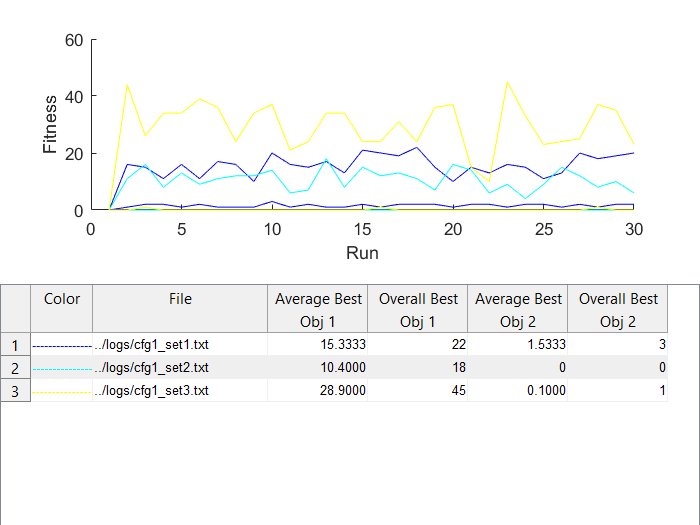
\includegraphics[width=5in]{assn1d_cfg1_bestfitness.png}
  \captionof{figure}{Best Per-Objective Fitness}
  \label{fig:cfg1_best}
\end{figure}
\begin{figure}[h]
	\centering
  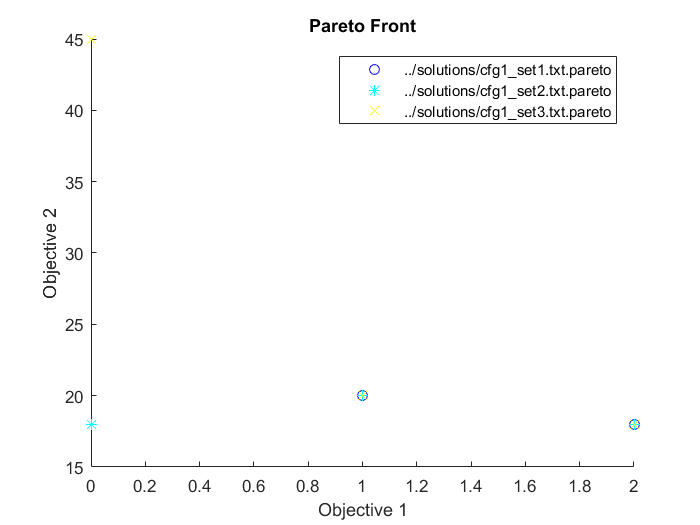
\includegraphics[width=4in]{assn1d_cfg1_pareto.png}
  \captionof{figure}{Pareto Fronts}
  \label{fig:cfg1_pareto}
\end{figure}

\section{Configuration 2}\label{sect:cfg2}

\section{Configuration 3}\label{sect:cfg3}

\section{Bonus 3}\label{sect:bonus3}

\end{document}